% Standalone version for quick TikZ annotation tuning
% Compile: pdflatex fig_contact_density_standalone.tex
% Use a PDF viewer with auto-refresh (e.g., Skim) for live preview
\documentclass[border=5pt]{standalone}
\usepackage{tikz}
\usetikzlibrary{arrows.meta, calc}
\usepackage{amsmath}
\usepackage{graphicx}
\graphicspath{{./}}

% Macro used in labels (self-contained, no dependency on main paper)
\newcommand{\Kzero}{K_0}

\begin{document}
\begin{tikzpicture}
  \def\imgW{3.4cm}   % image width — tune for standalone preview
  \def\gap{1pt}
  \def\rowgap{12pt}

  % --- Row 1: K0=0.5 ---
  \node[anchor=north west, inner sep=0] (a1) at (0,0)
    {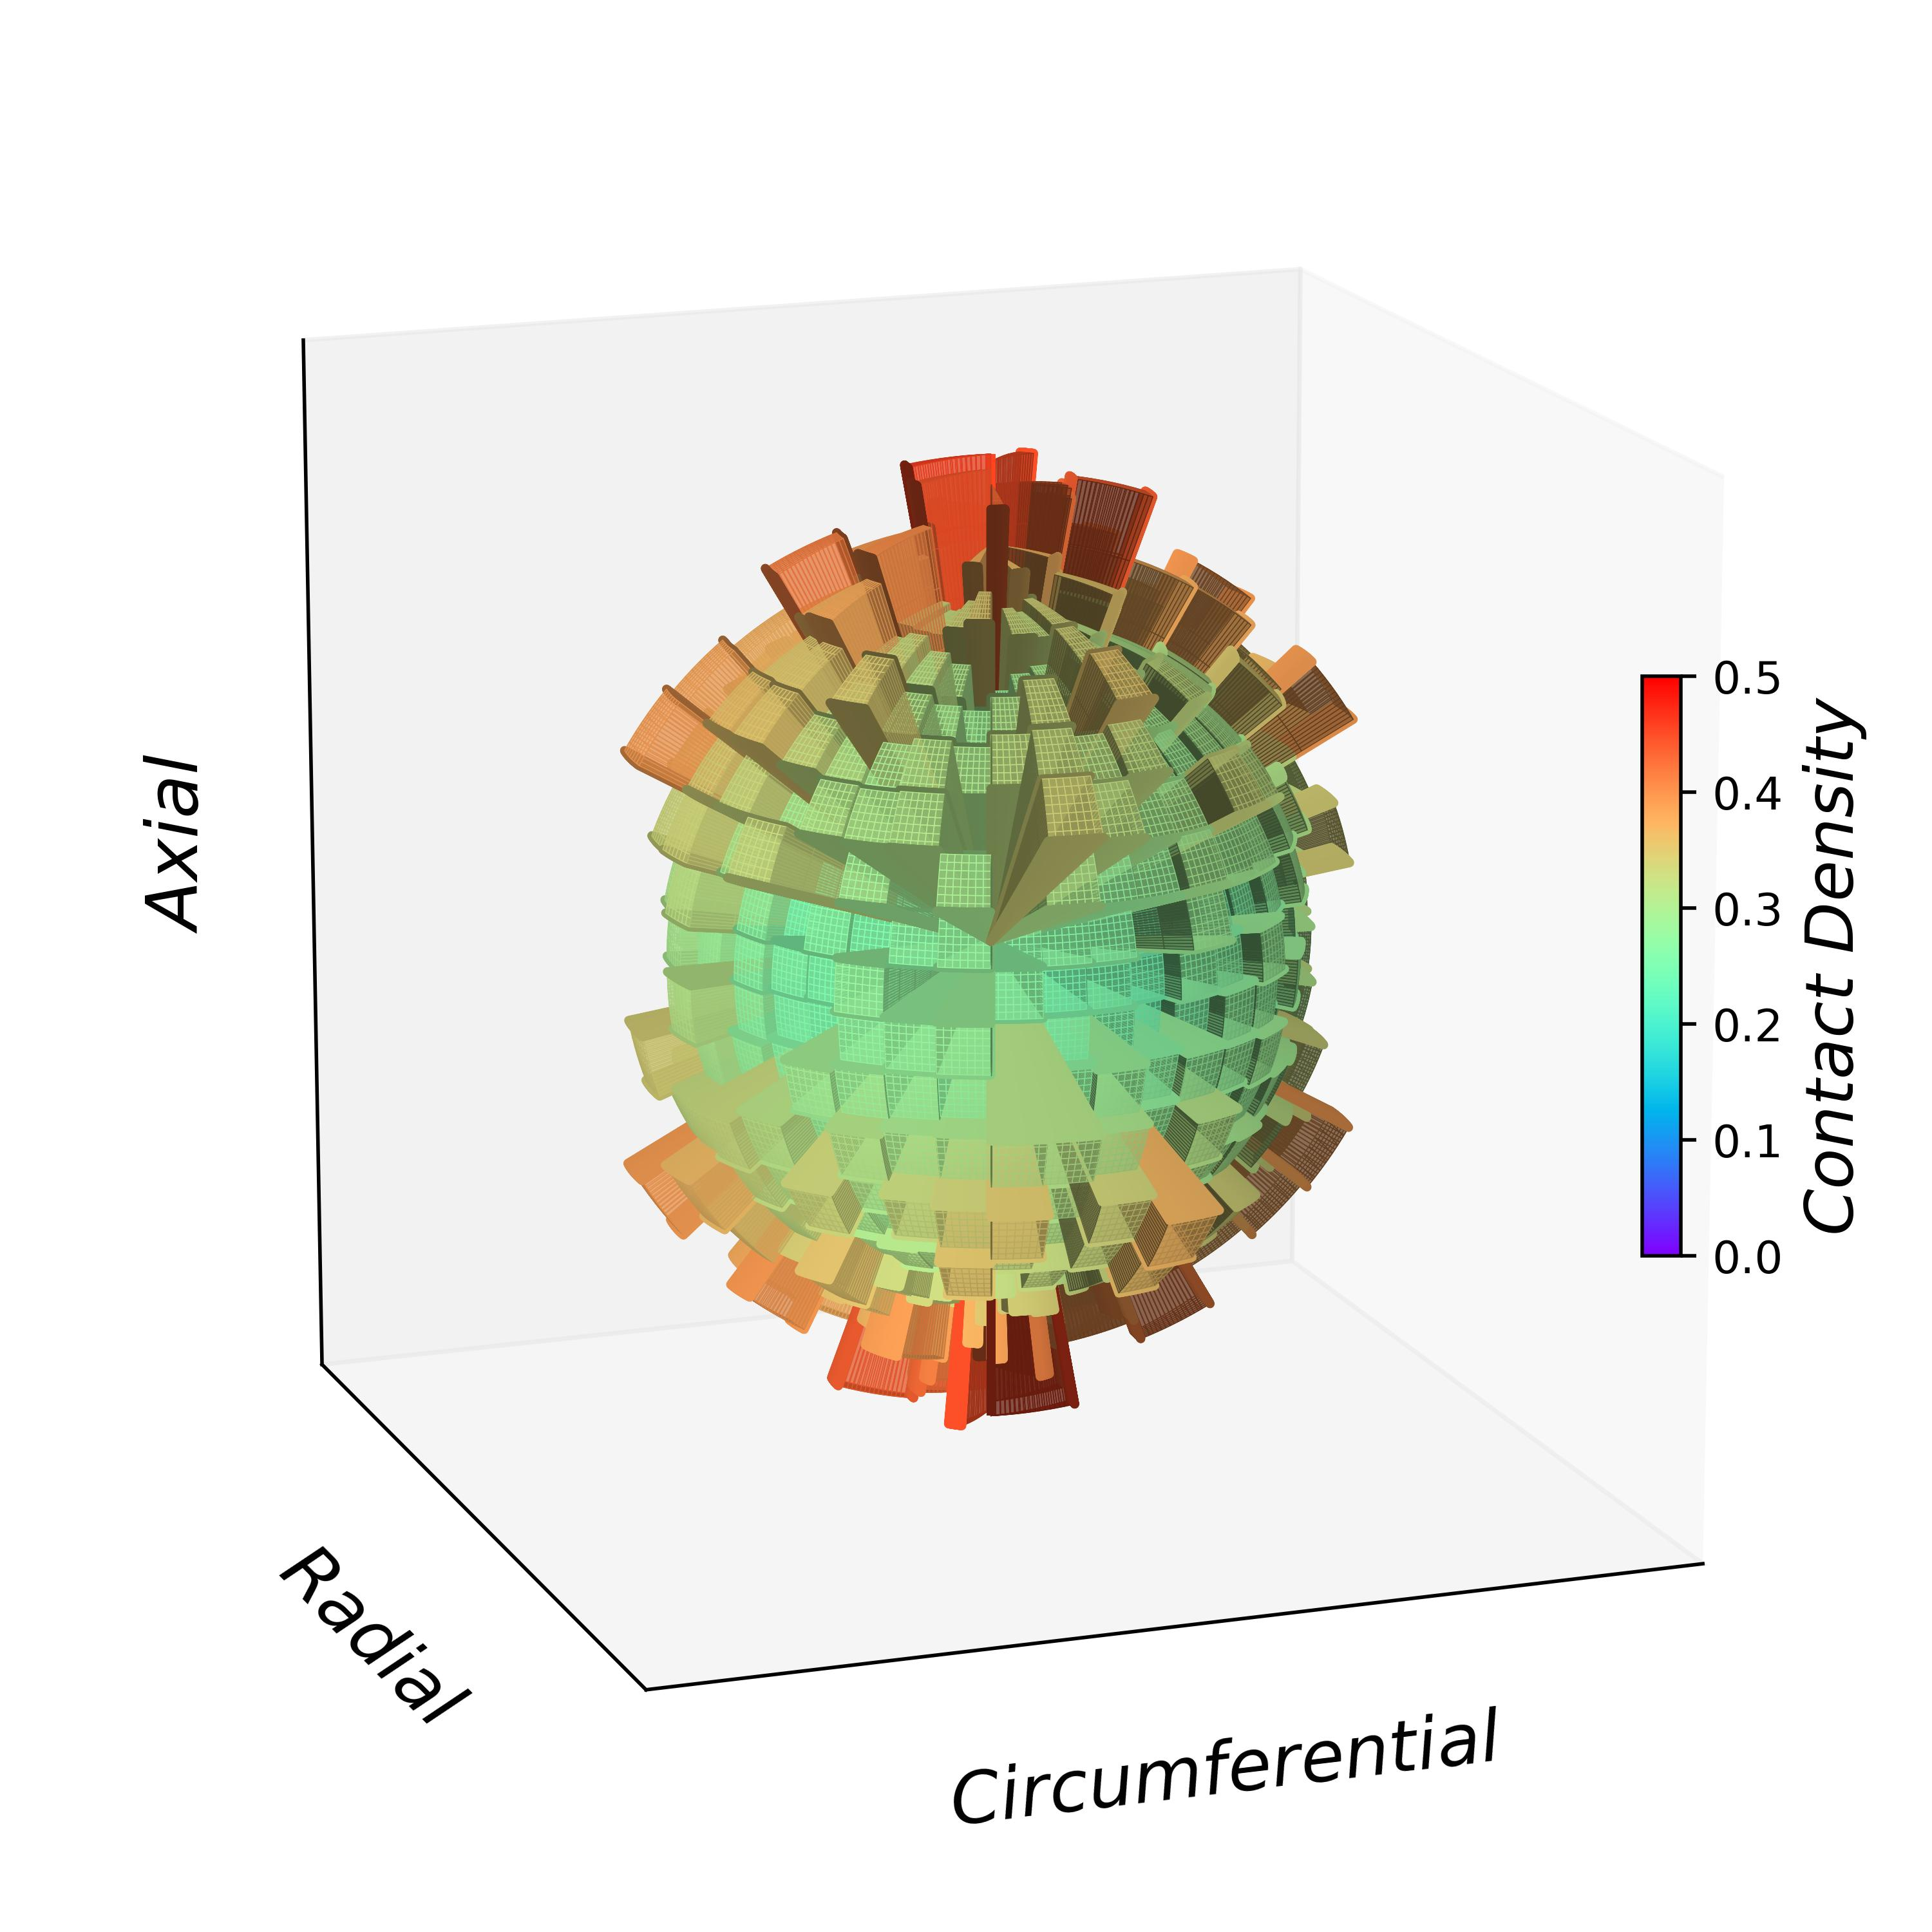
\includegraphics[width=\imgW]{contact_density_k0_05_t0.png}};
  \node[font=\small, anchor=south] at (a1.north) {$N/N_L = 0.00$};
  \node[anchor=north west, inner sep=0] (a2) at ([xshift=\gap]a1.north east)
    {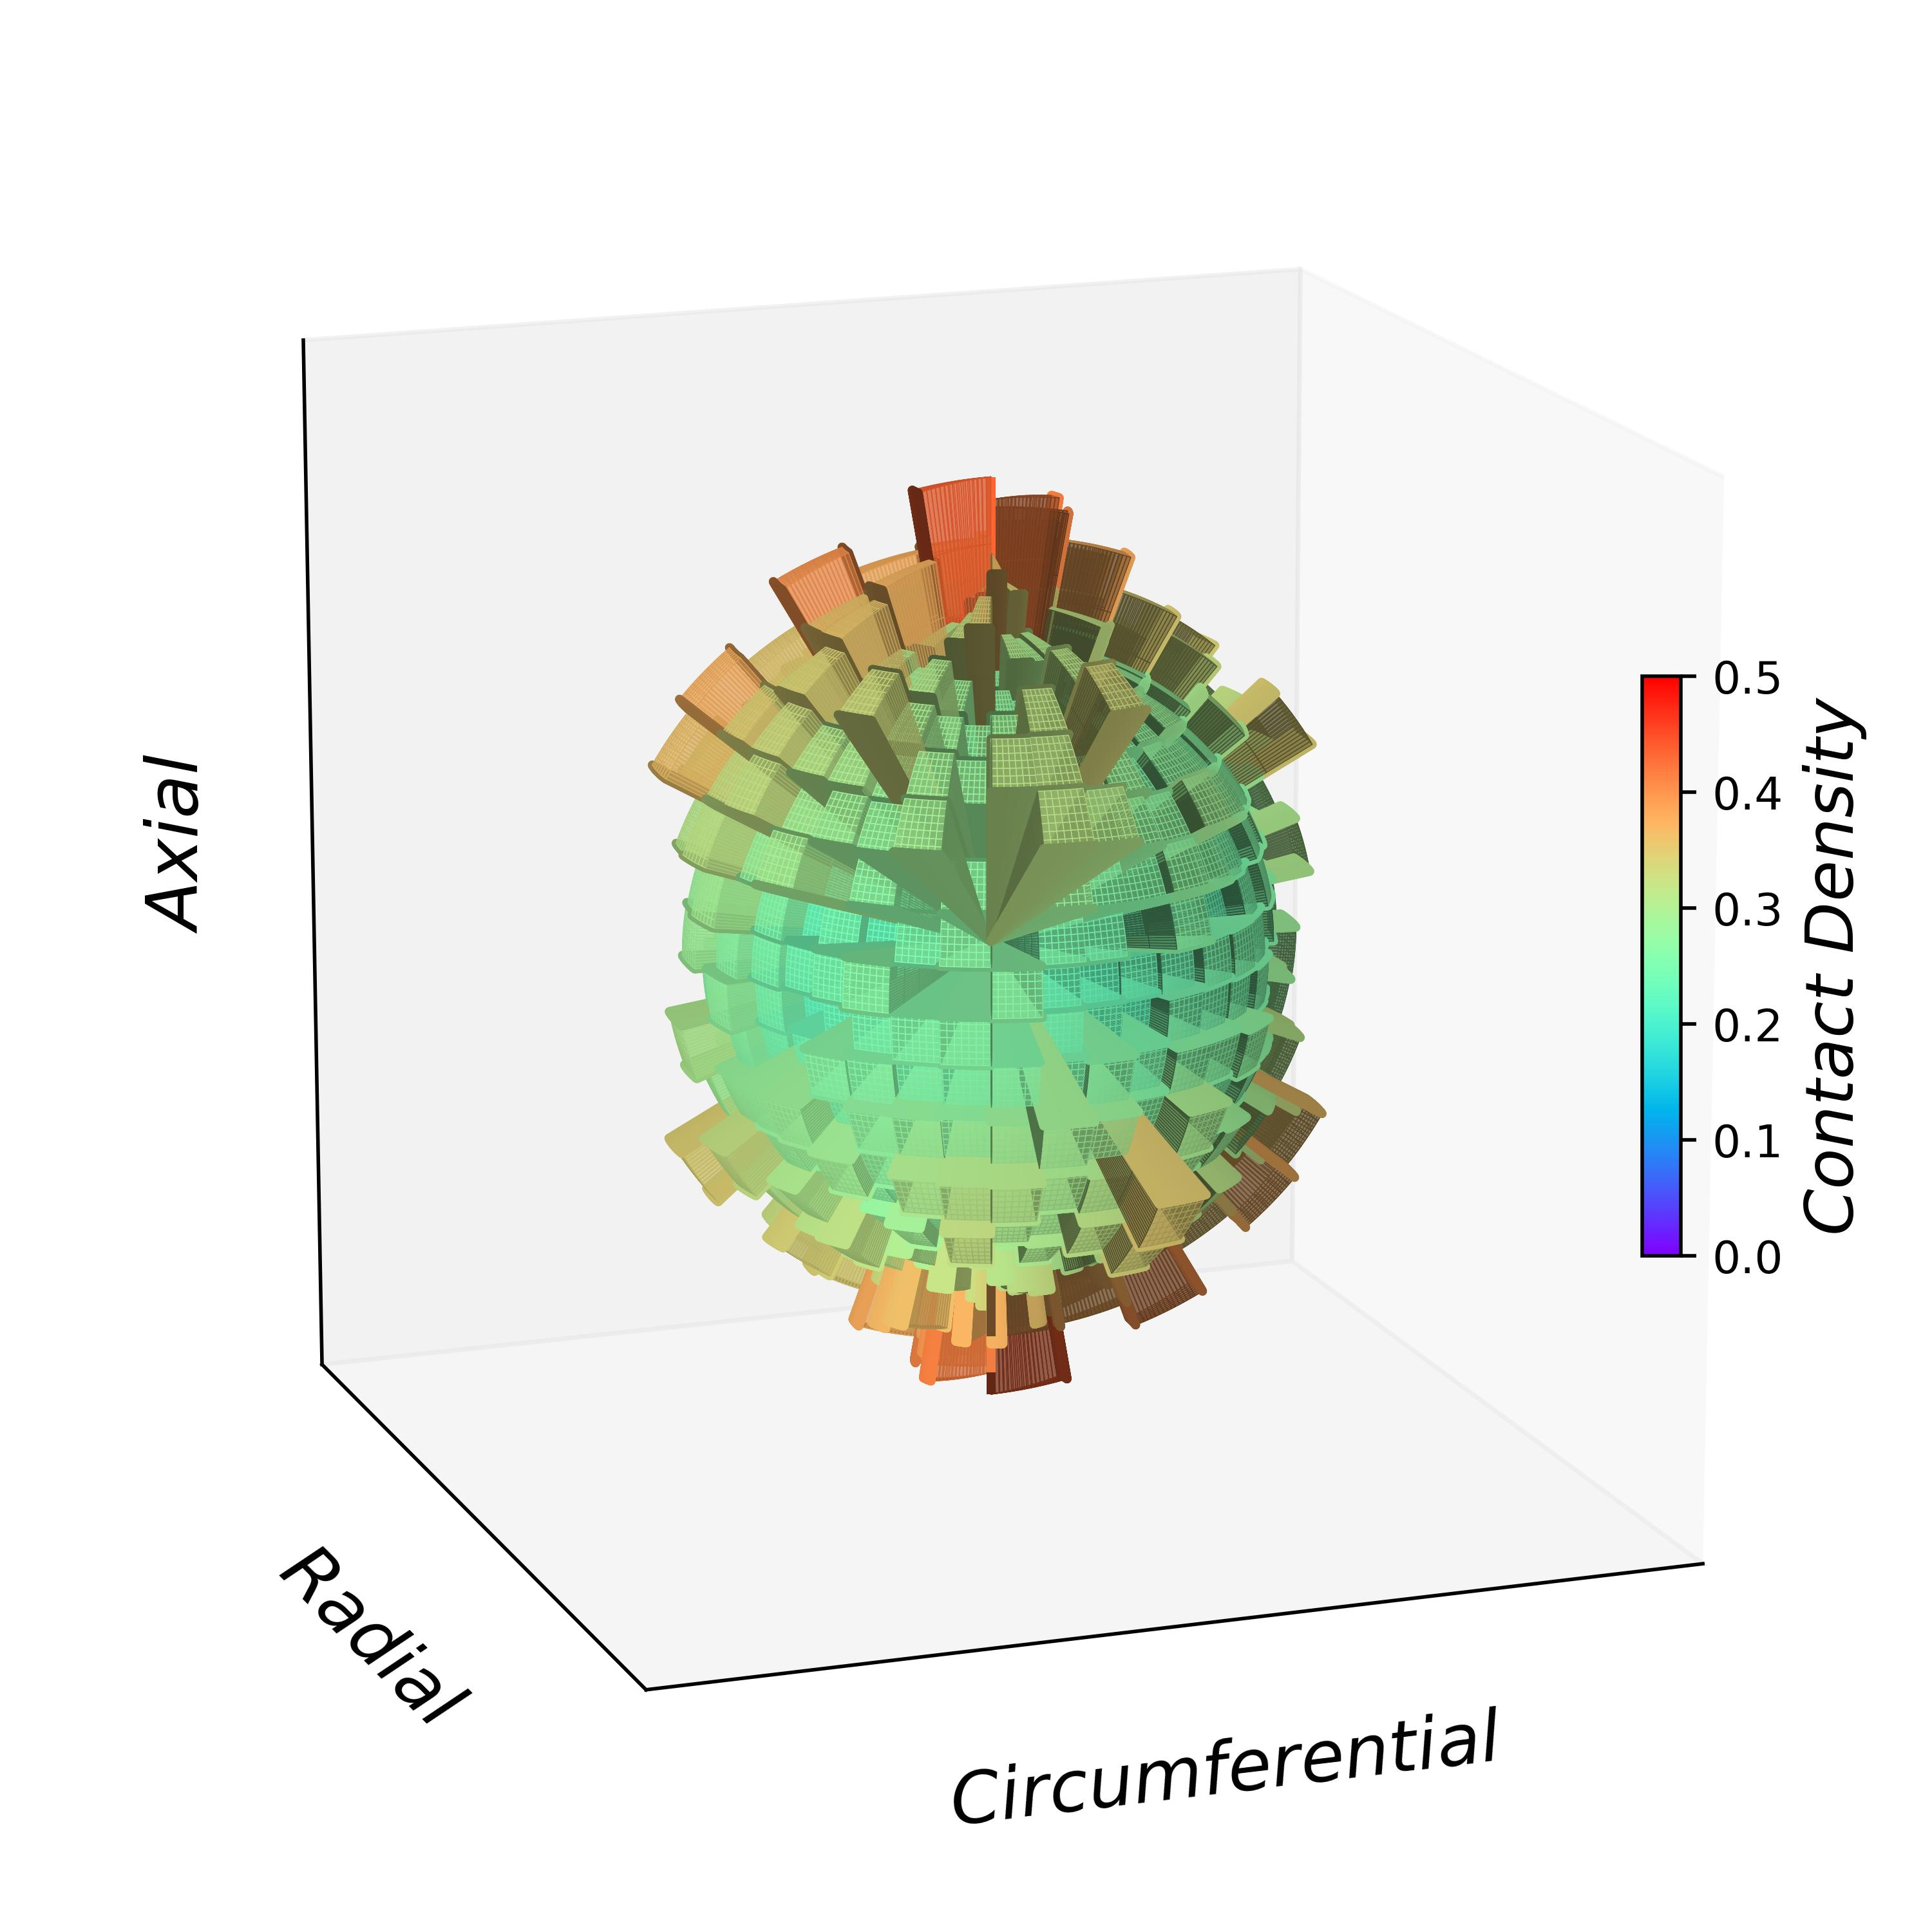
\includegraphics[width=\imgW]{contact_density_k0_05_t302.png}};
  \node[font=\small, anchor=south] at (a2.north) {$N/N_L \approx 0.61$};
  \node[anchor=north west, inner sep=0] (a3) at ([xshift=\gap]a2.north east)
    {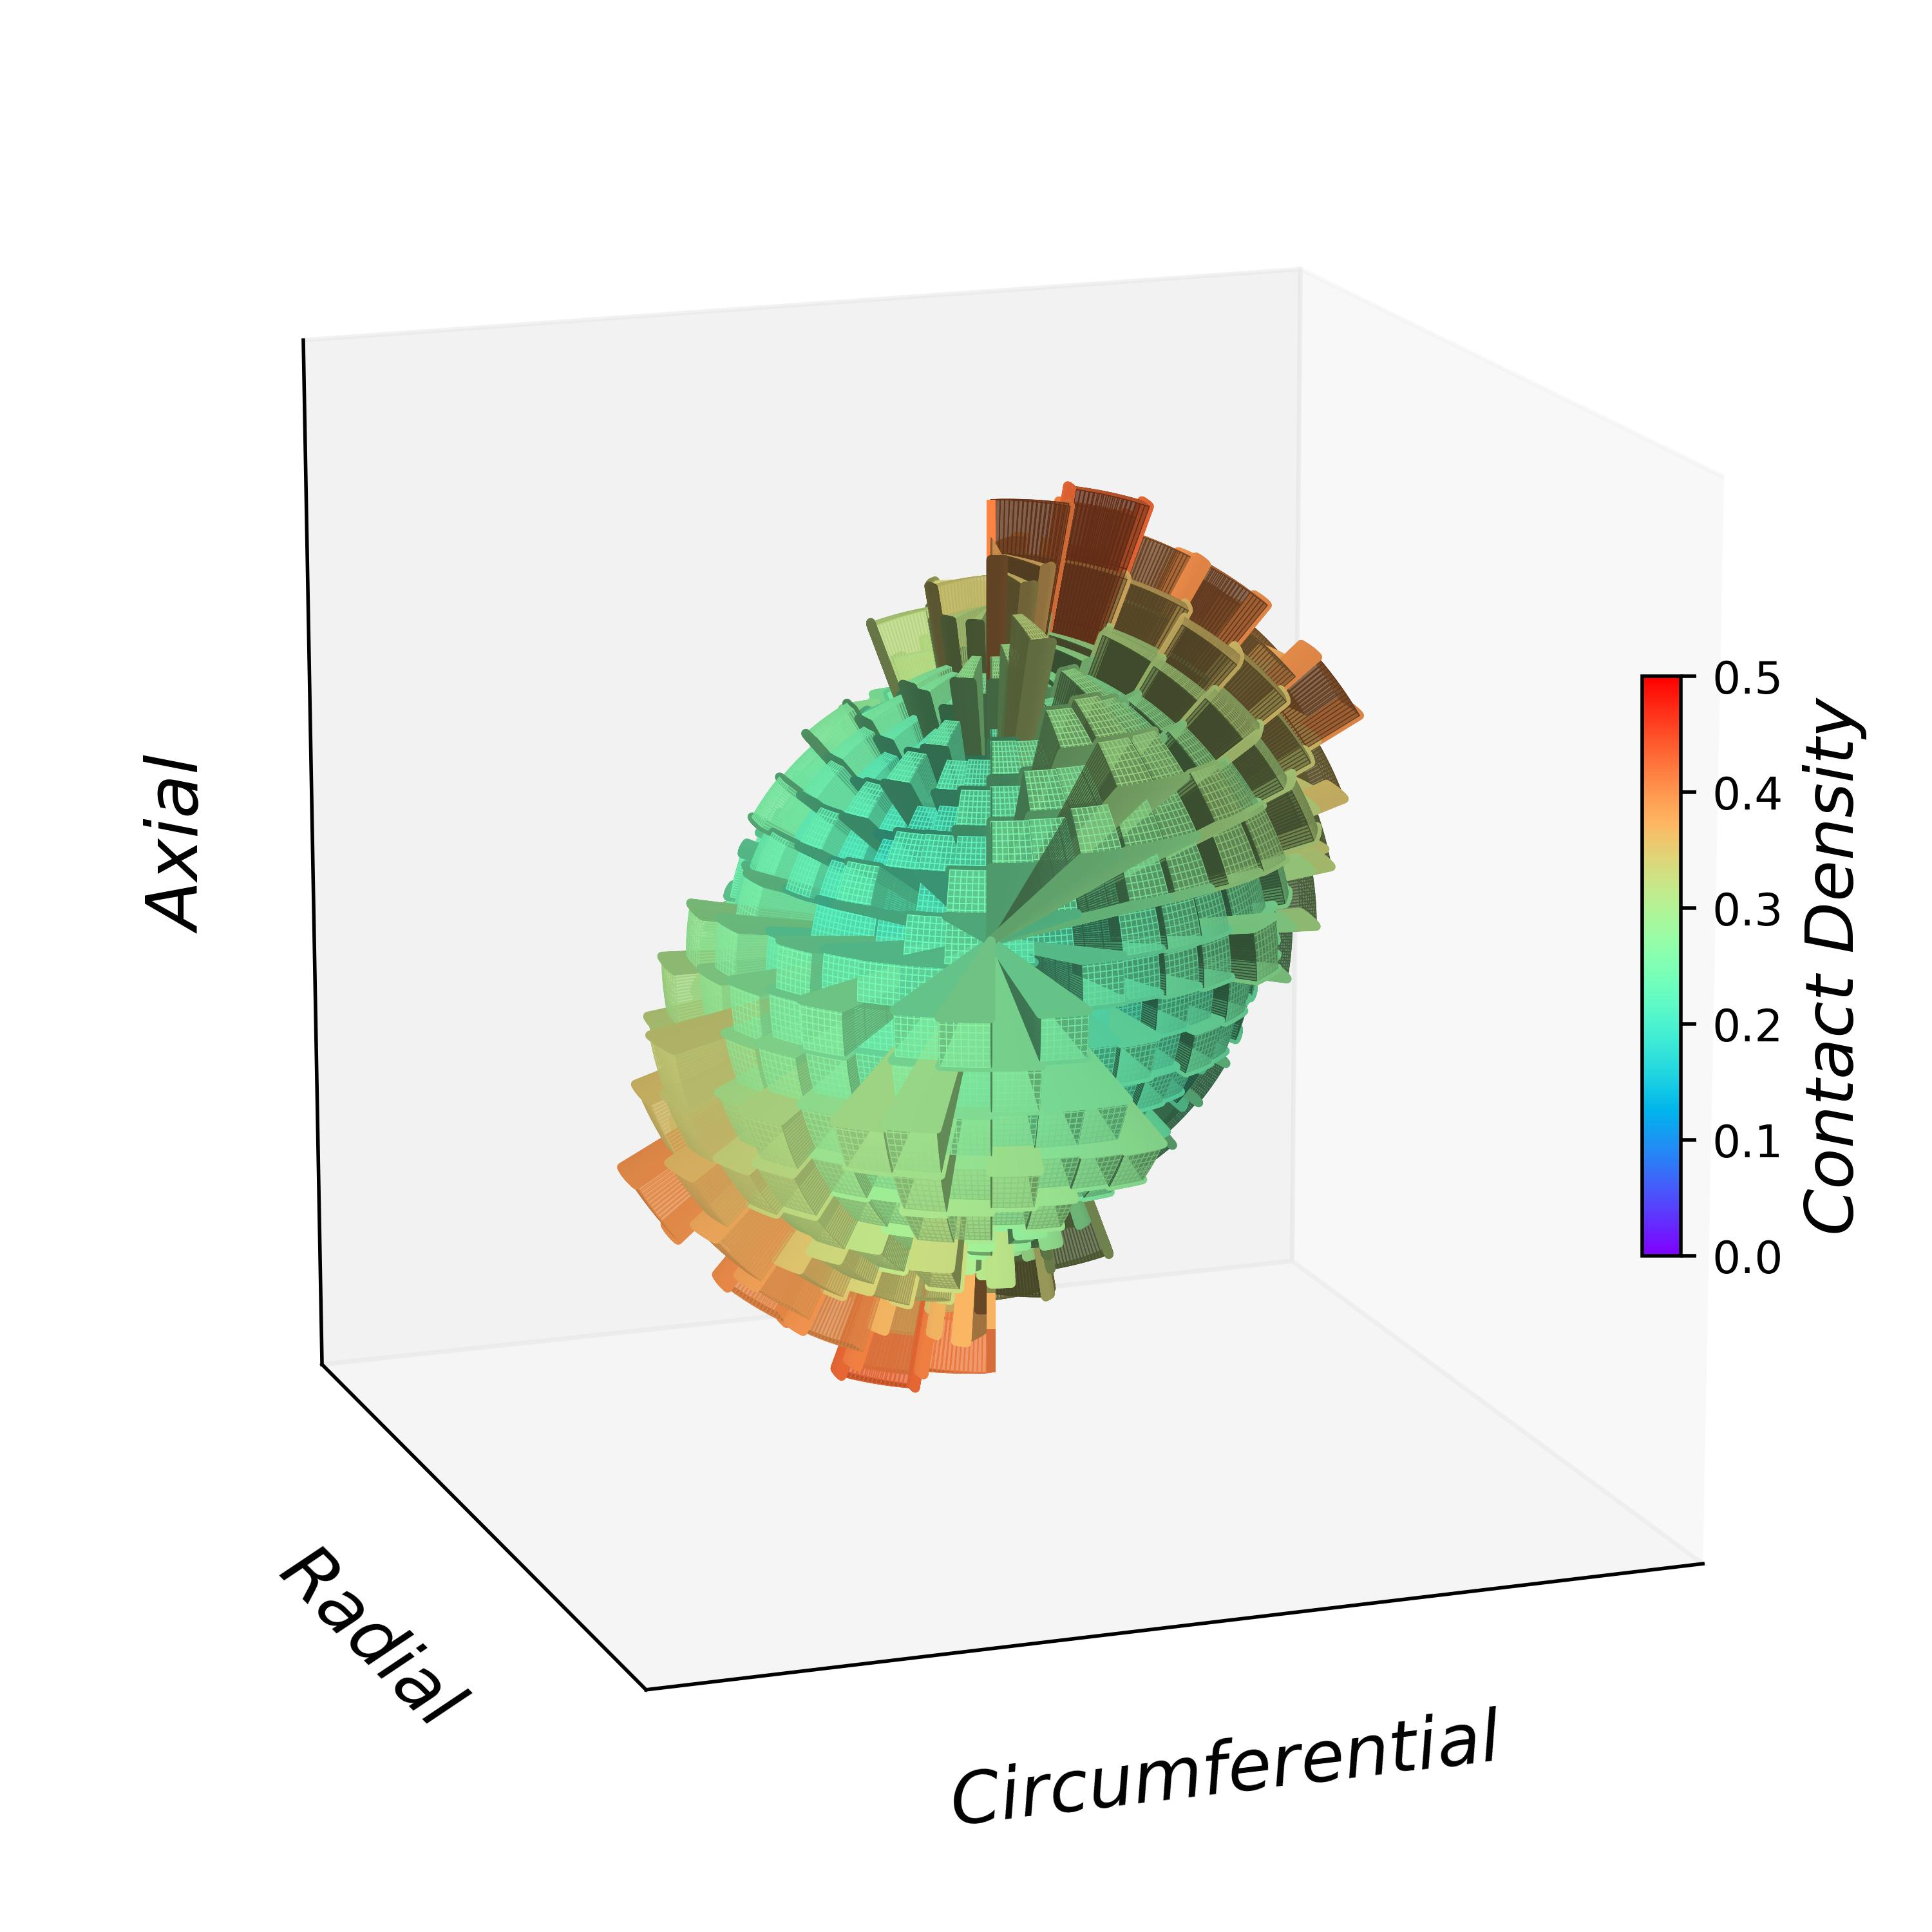
\includegraphics[width=\imgW]{contact_density_k0_05_t523.png}};
  \node[font=\small, anchor=south] at (a3.north) {$N/N_L \approx 1.05$};
  \node[anchor=north west, inner sep=0] (a4) at ([xshift=\gap]a3.north east)
    {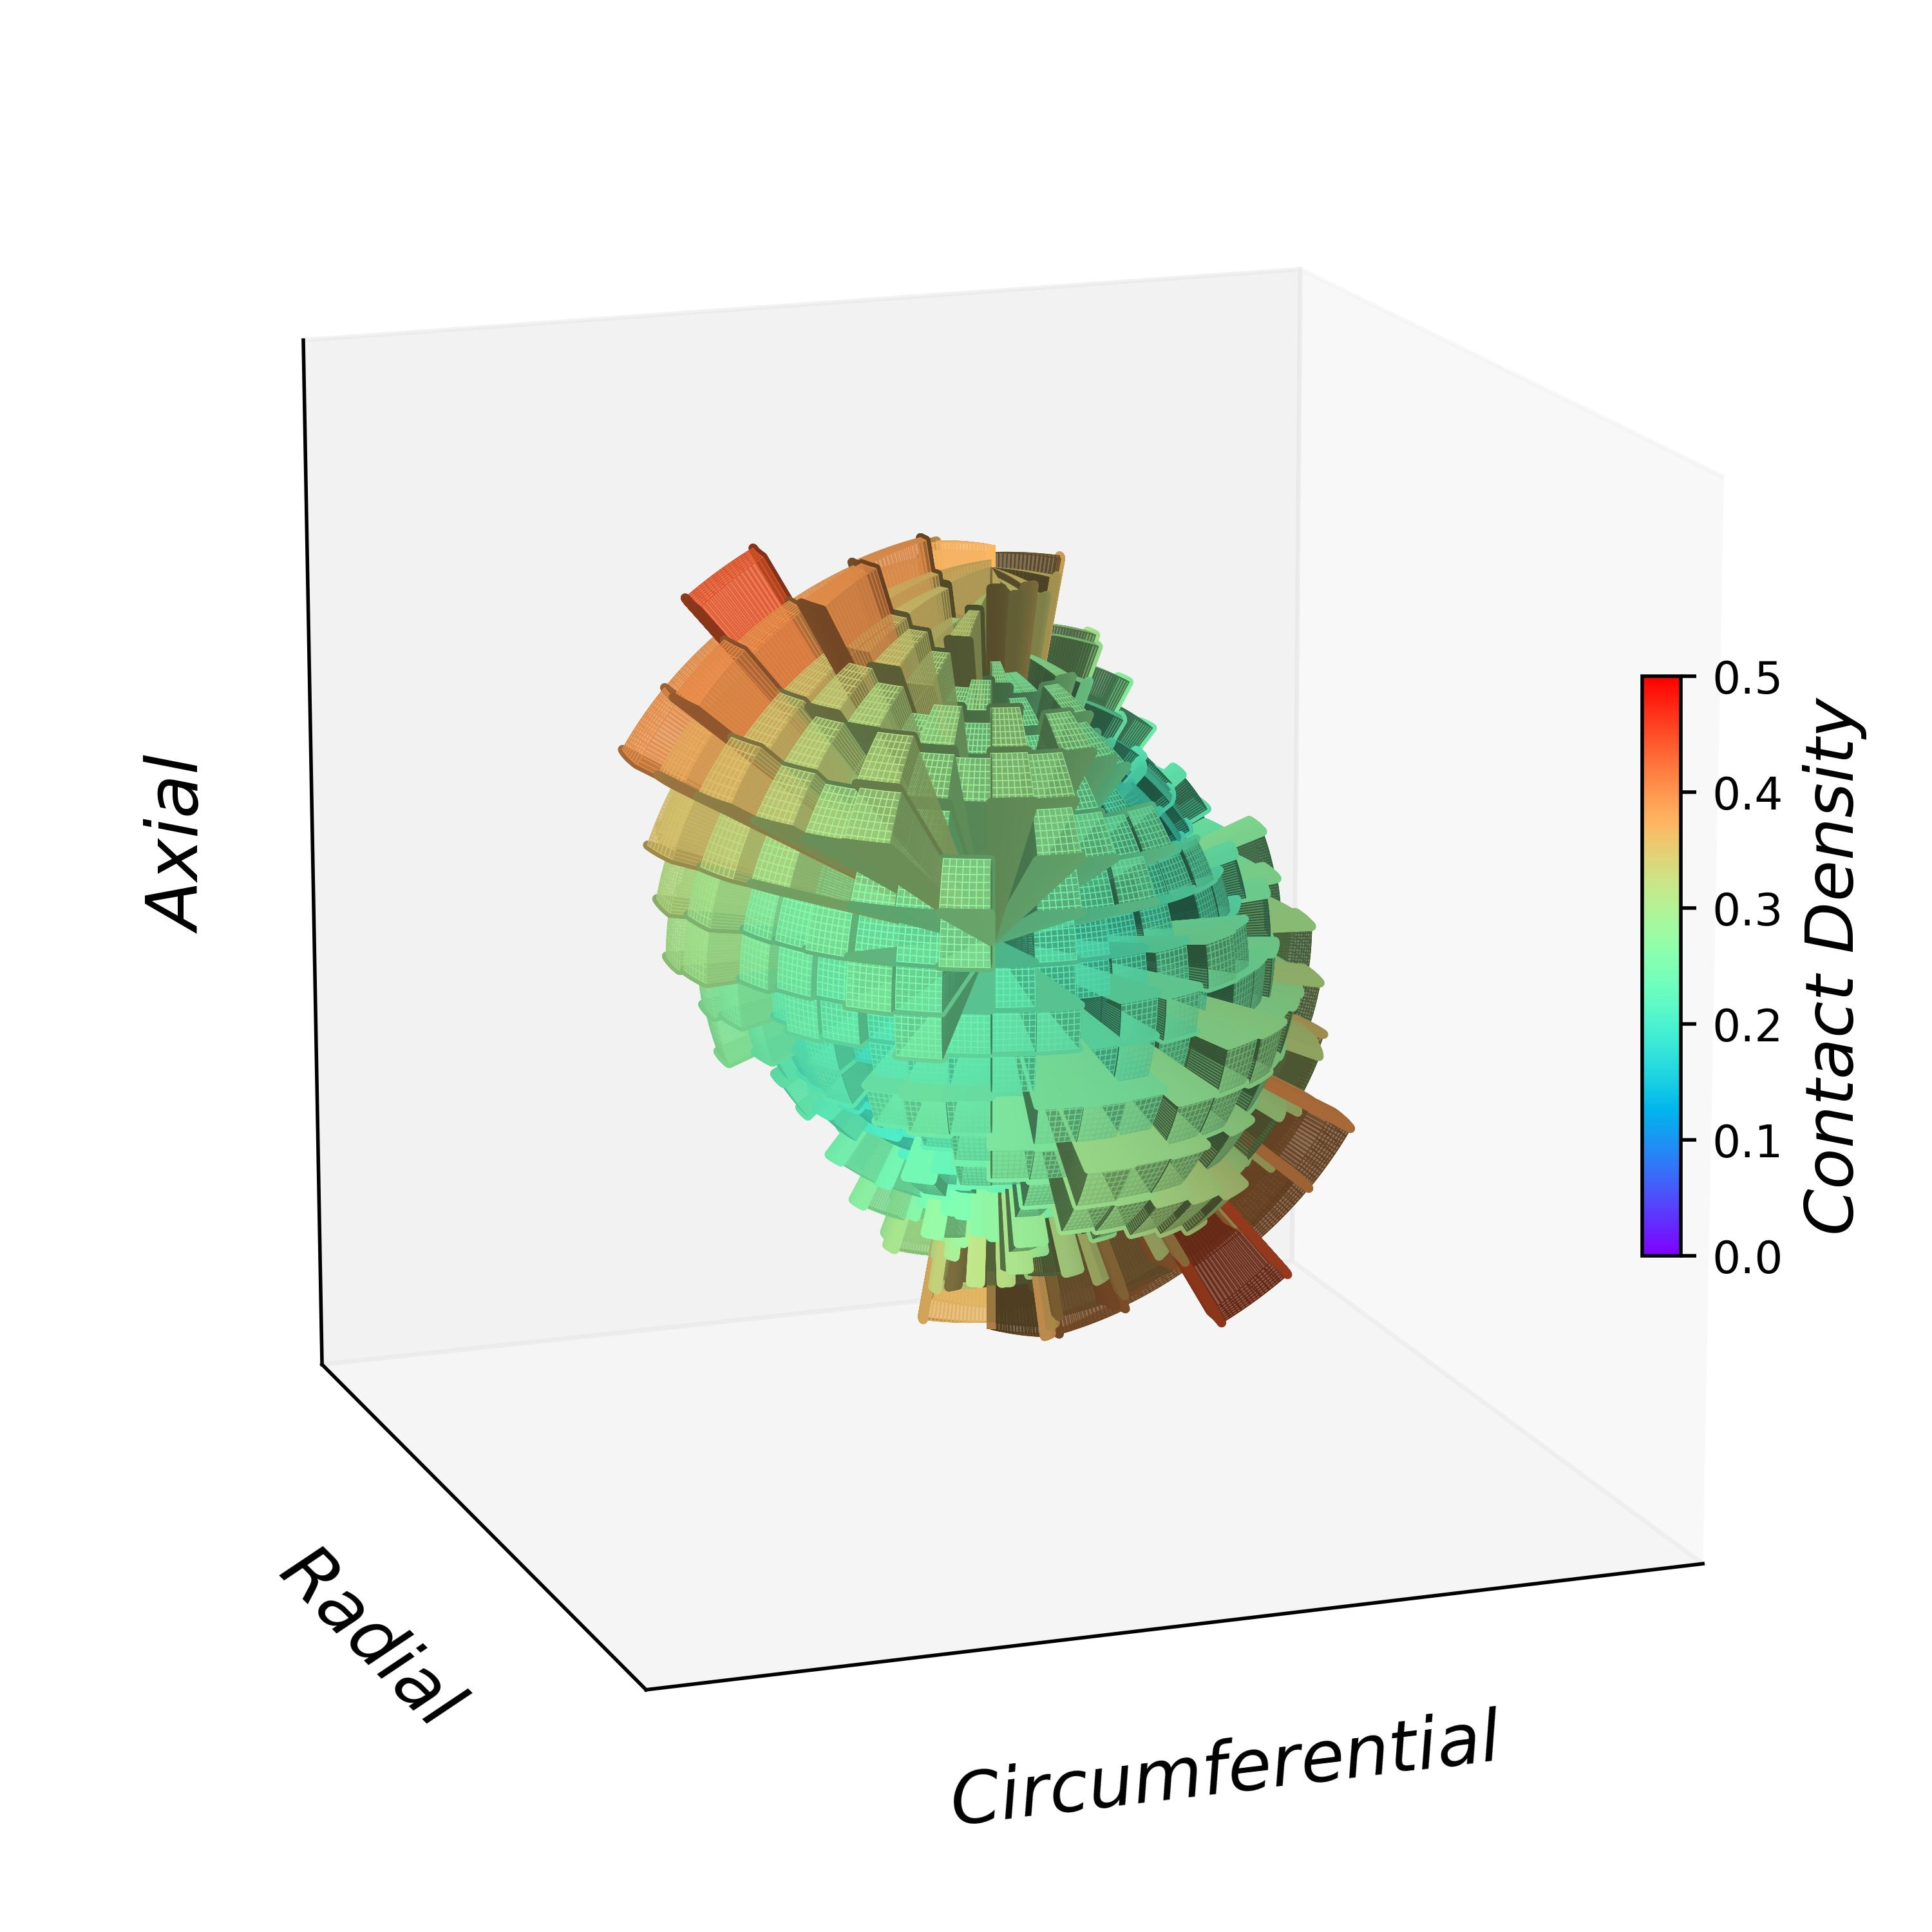
\includegraphics[width=\imgW]{contact_density_k0_05_t529.png}};
  \node[font=\small, anchor=south] at (a4.north) {$N/N_L \approx 1.07$};

  % --- Axis labels on first image (a1) ---
  % Anchor at bottom-left of a1; adjust offsets to taste
  \coordinate (axO) at ([xshift=6pt, yshift=12pt]a1.south west);
  \draw[->, thick] (axO) -- ++(0, 14pt)   node[font=\scriptsize, right, inner sep=1pt] {$z$};
  \draw[->, thick] (axO) -- ++(16pt, 2pt) node[font=\scriptsize, right, inner sep=1pt] {$\theta$};
  \draw[->, thick] (axO) -- ++(8pt, -8pt) node[font=\scriptsize, right, inner sep=1pt] {$r$};

  % K0=0.5 label
  \path (a1.south) -- (a4.south) coordinate[midway] (row1mid);
  \node[font=\scriptsize, anchor=north] at ([yshift=-1pt]row1mid) {$\Kzero{} = 0.5$};

  % --- Row 2: K0=2.0 ---
  \node[anchor=north west, inner sep=0] (b1) at ([yshift=-\rowgap]a1.south west)
    {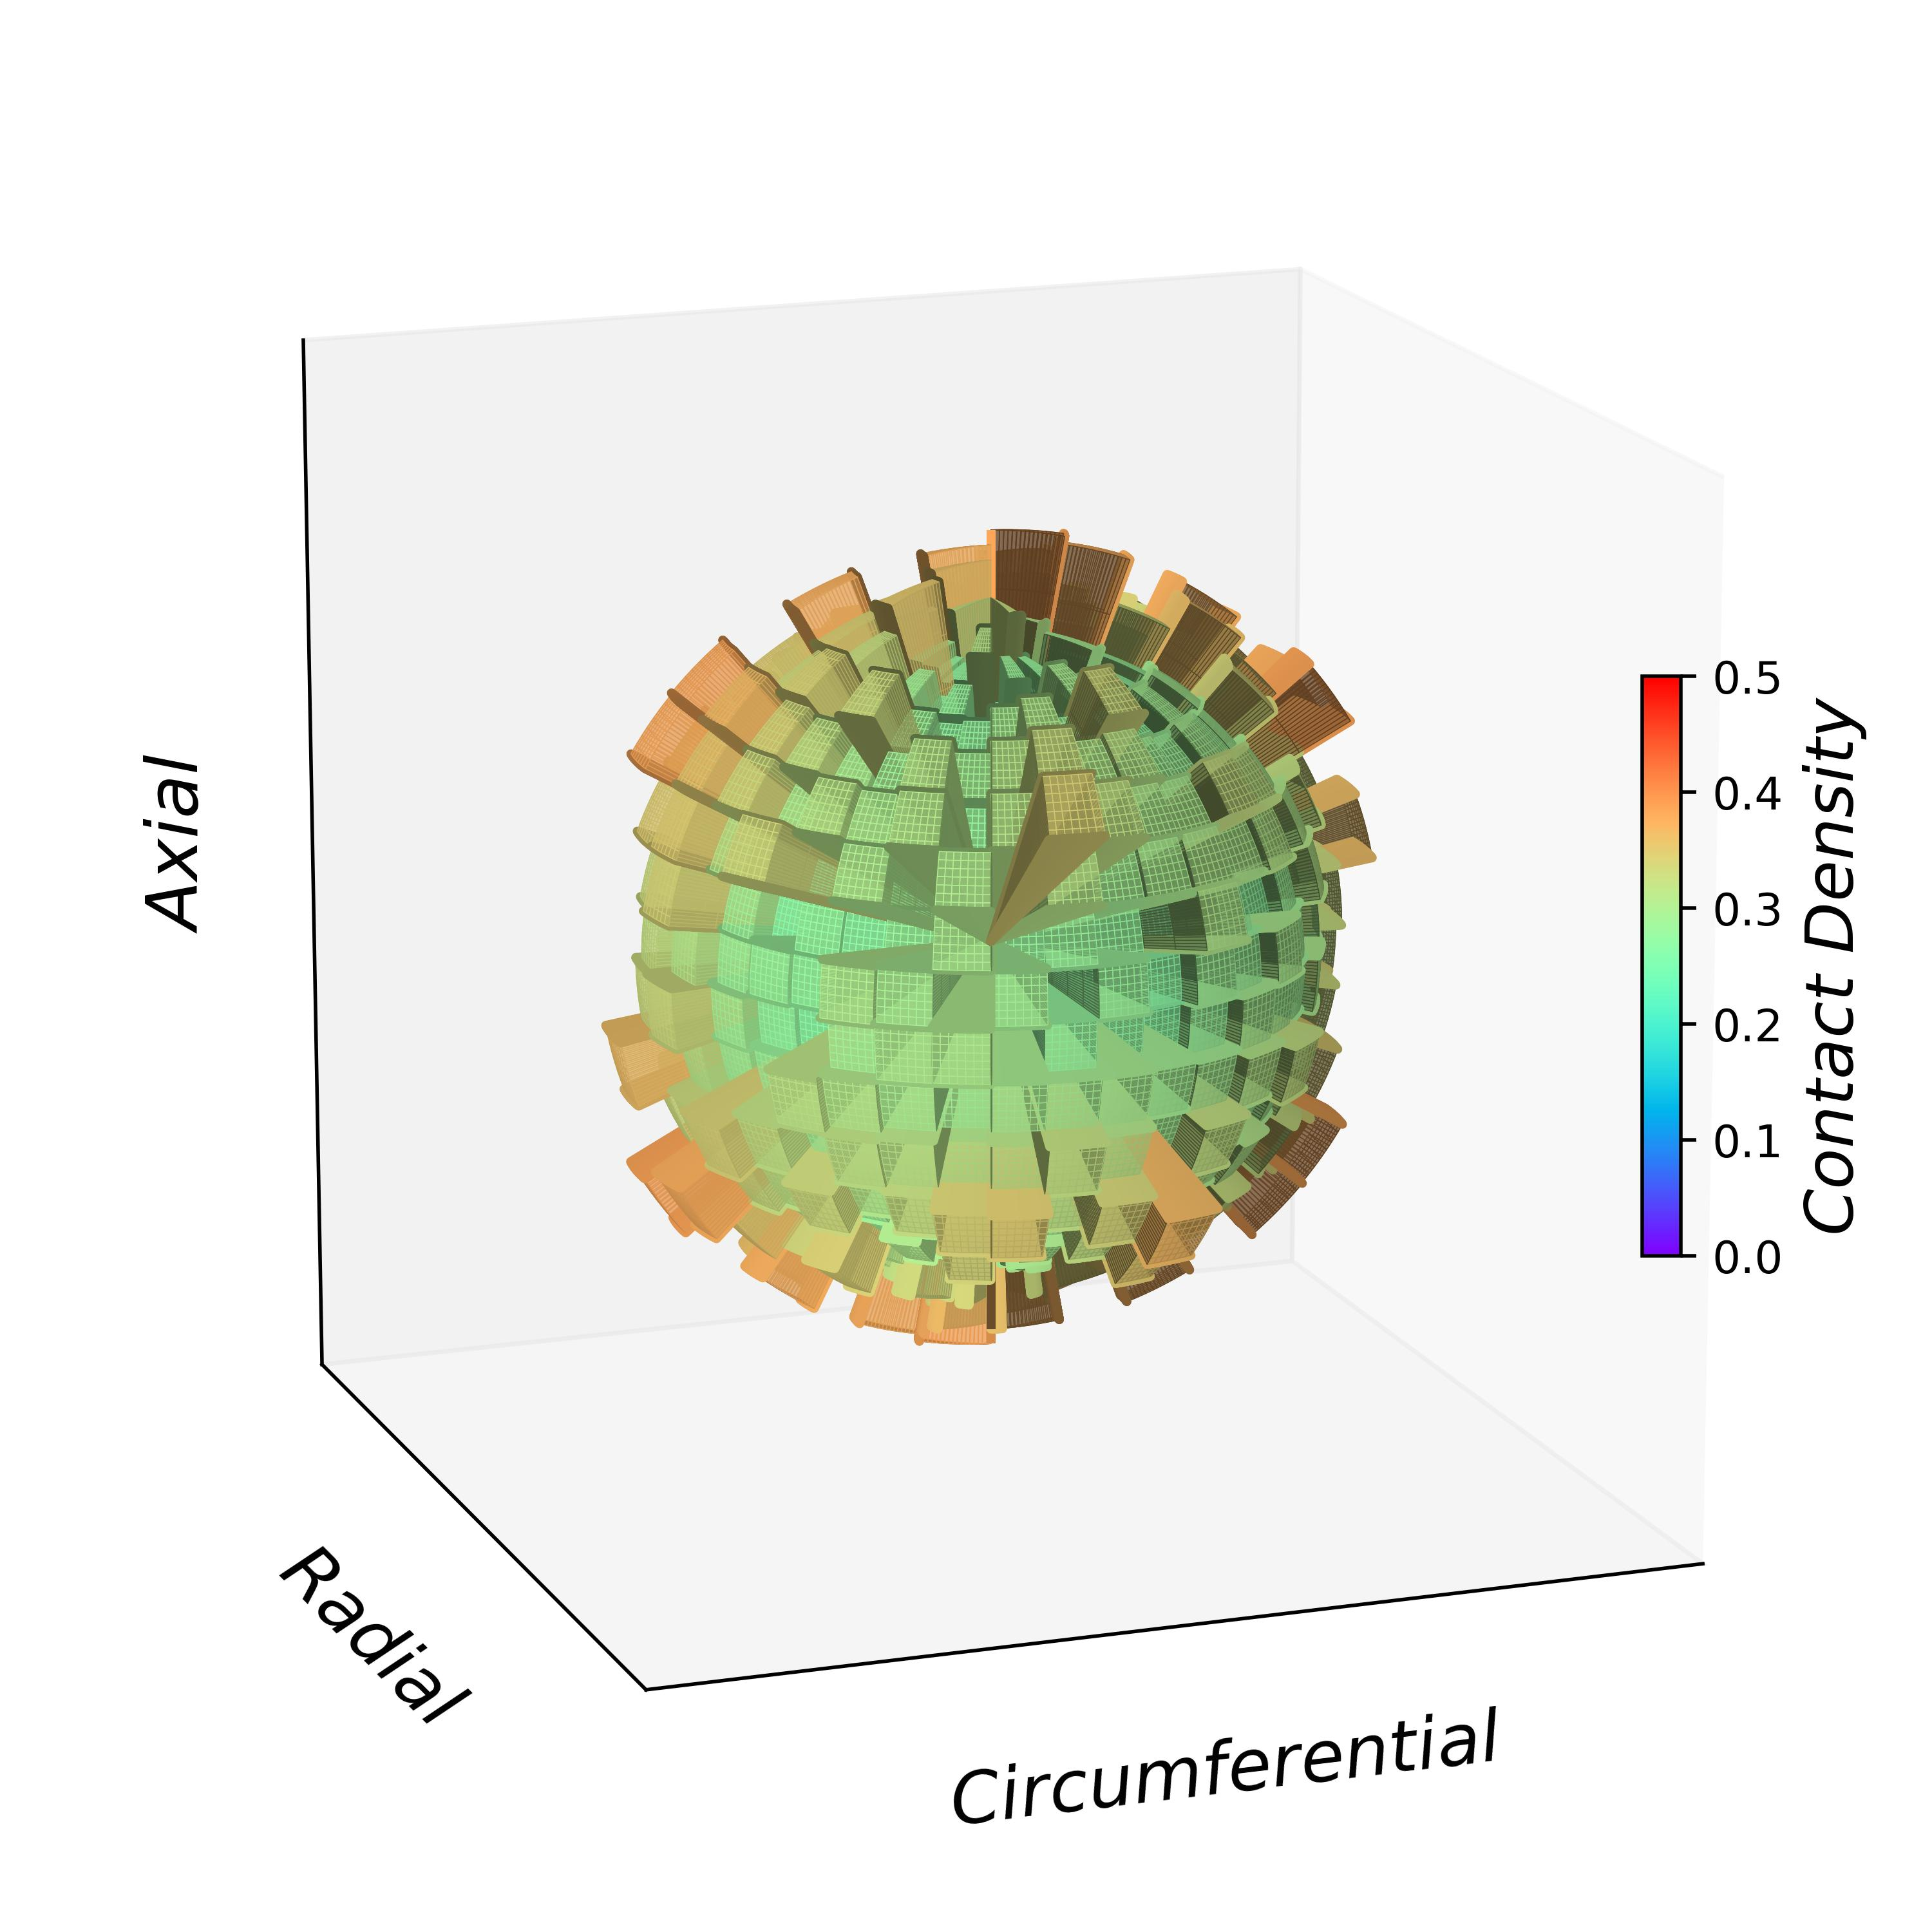
\includegraphics[width=\imgW]{contact_density_k0_20_t0.png}};
  \node[anchor=north west, inner sep=0] (b2) at ([xshift=\gap]b1.north east)
    {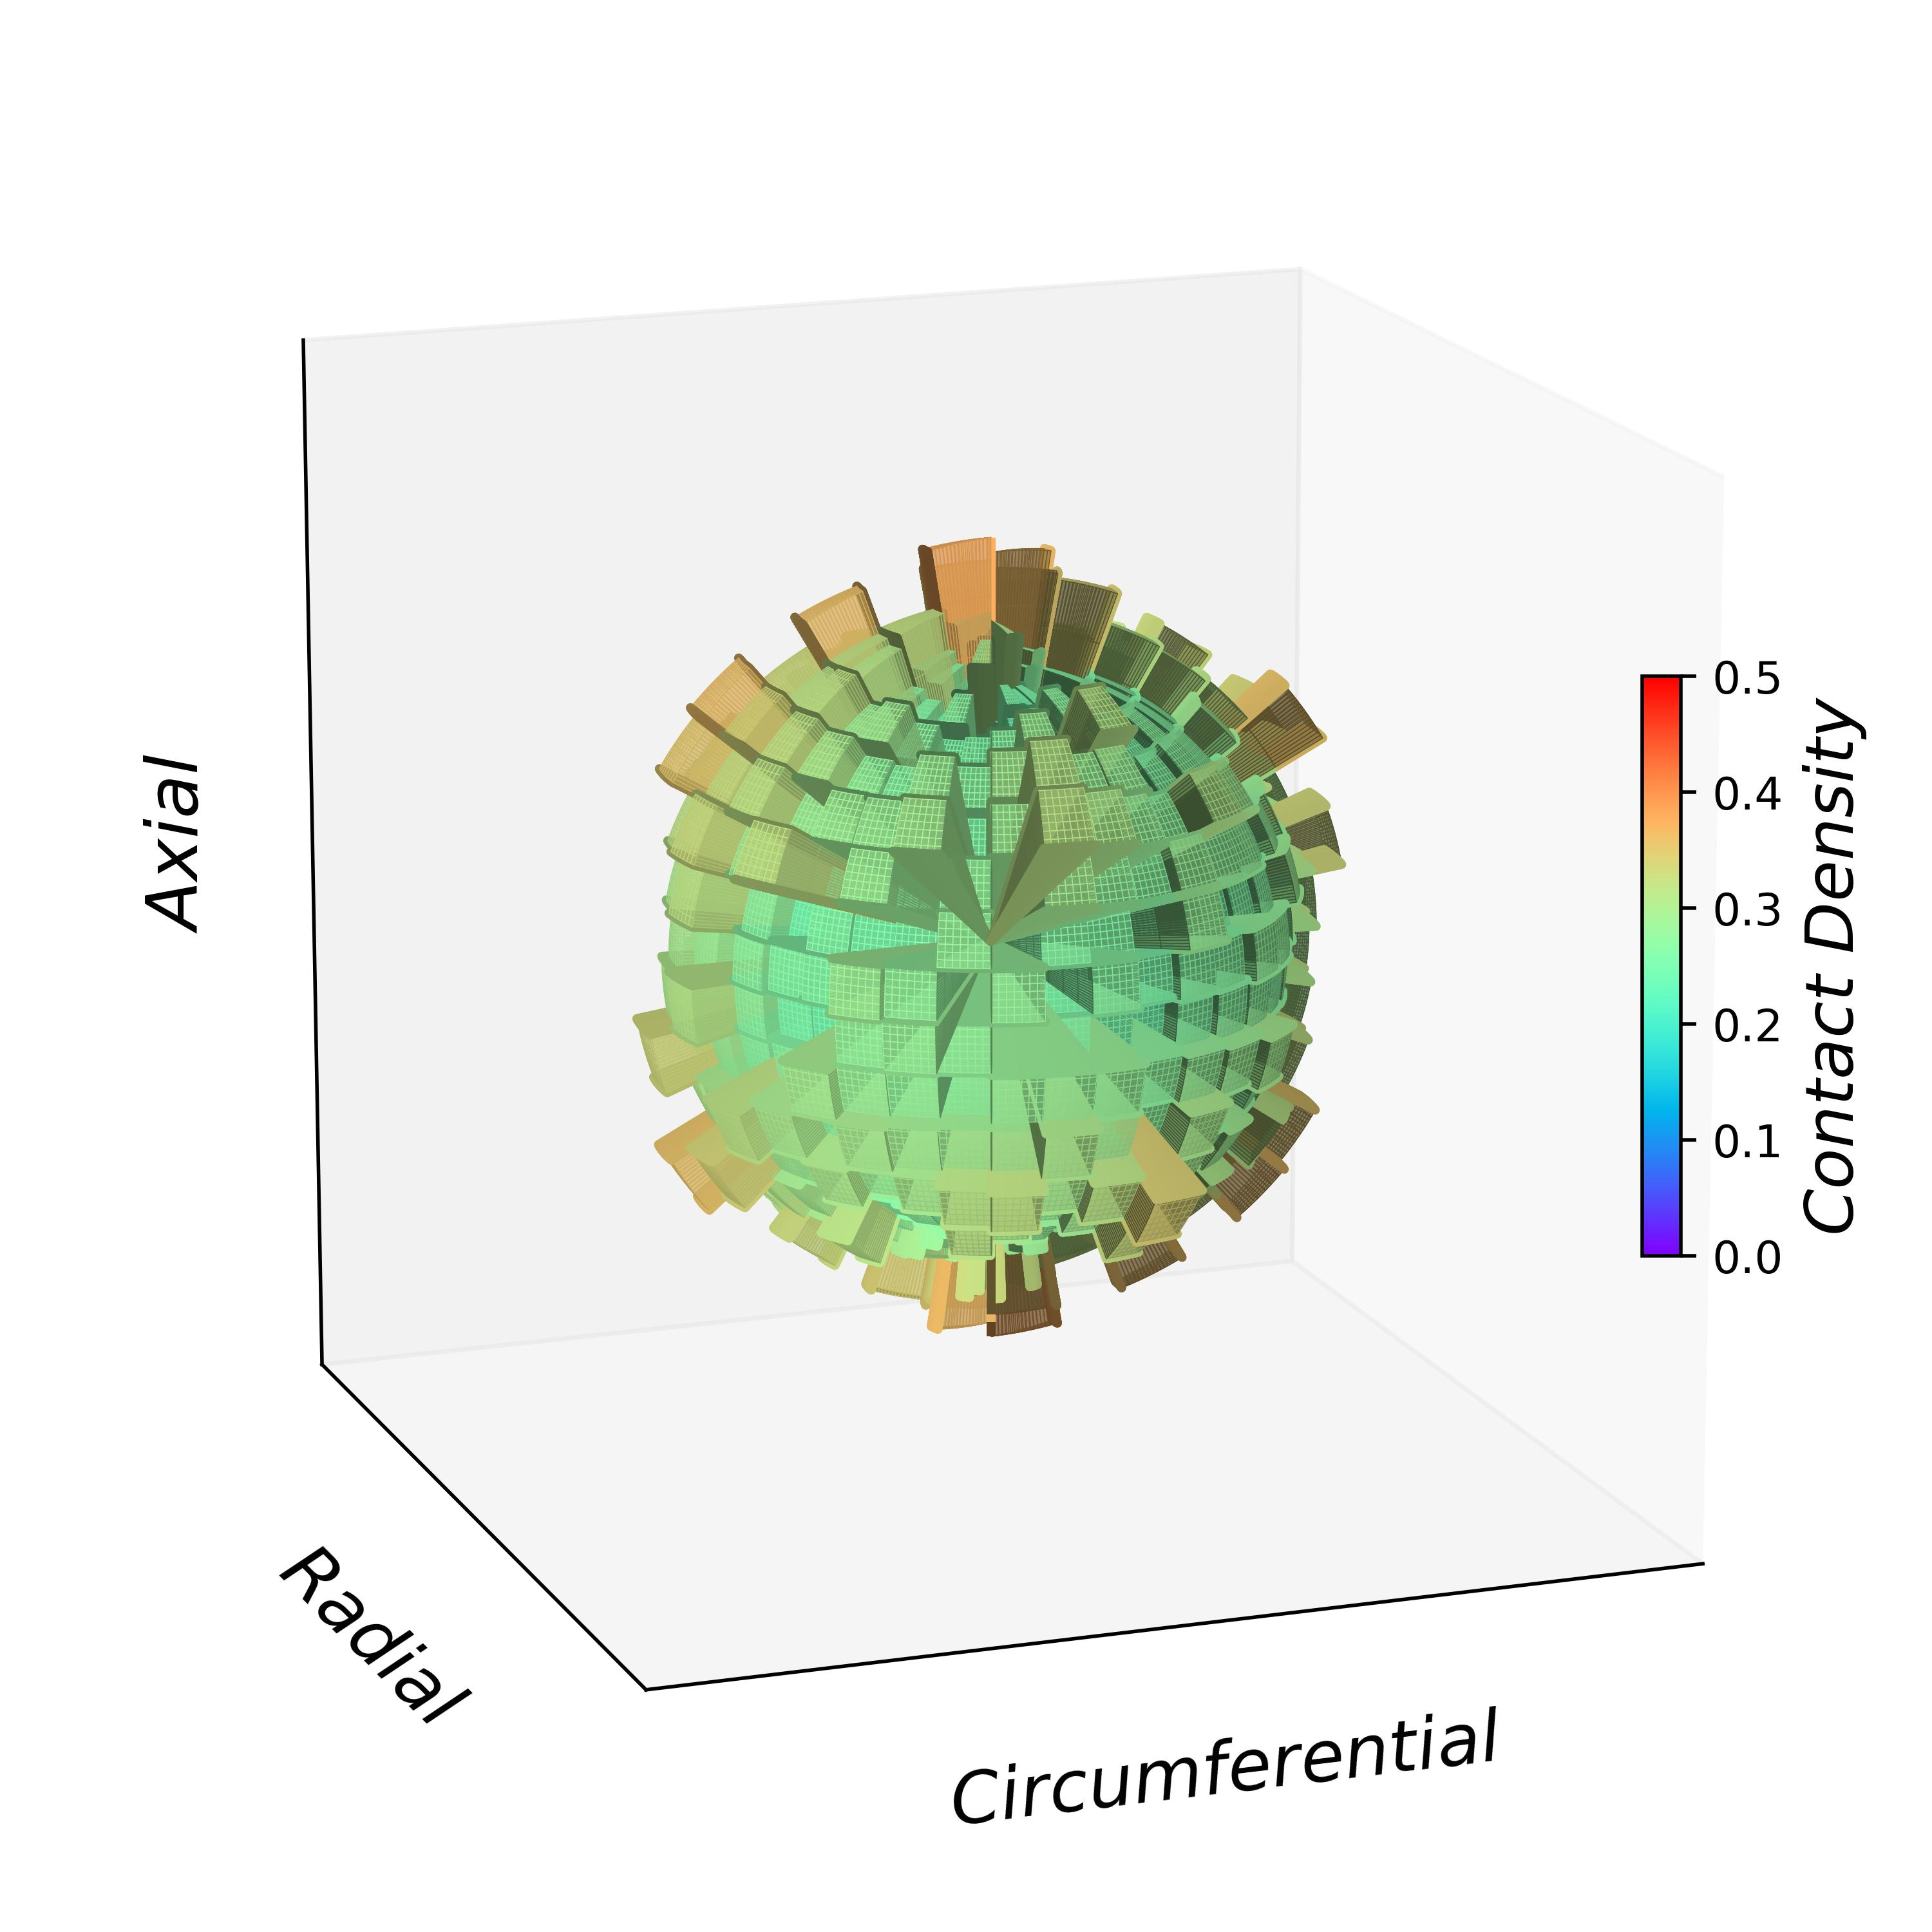
\includegraphics[width=\imgW]{contact_density_k0_20_t226.png}};
  \node[anchor=north west, inner sep=0] (b3) at ([xshift=\gap]b2.north east)
    {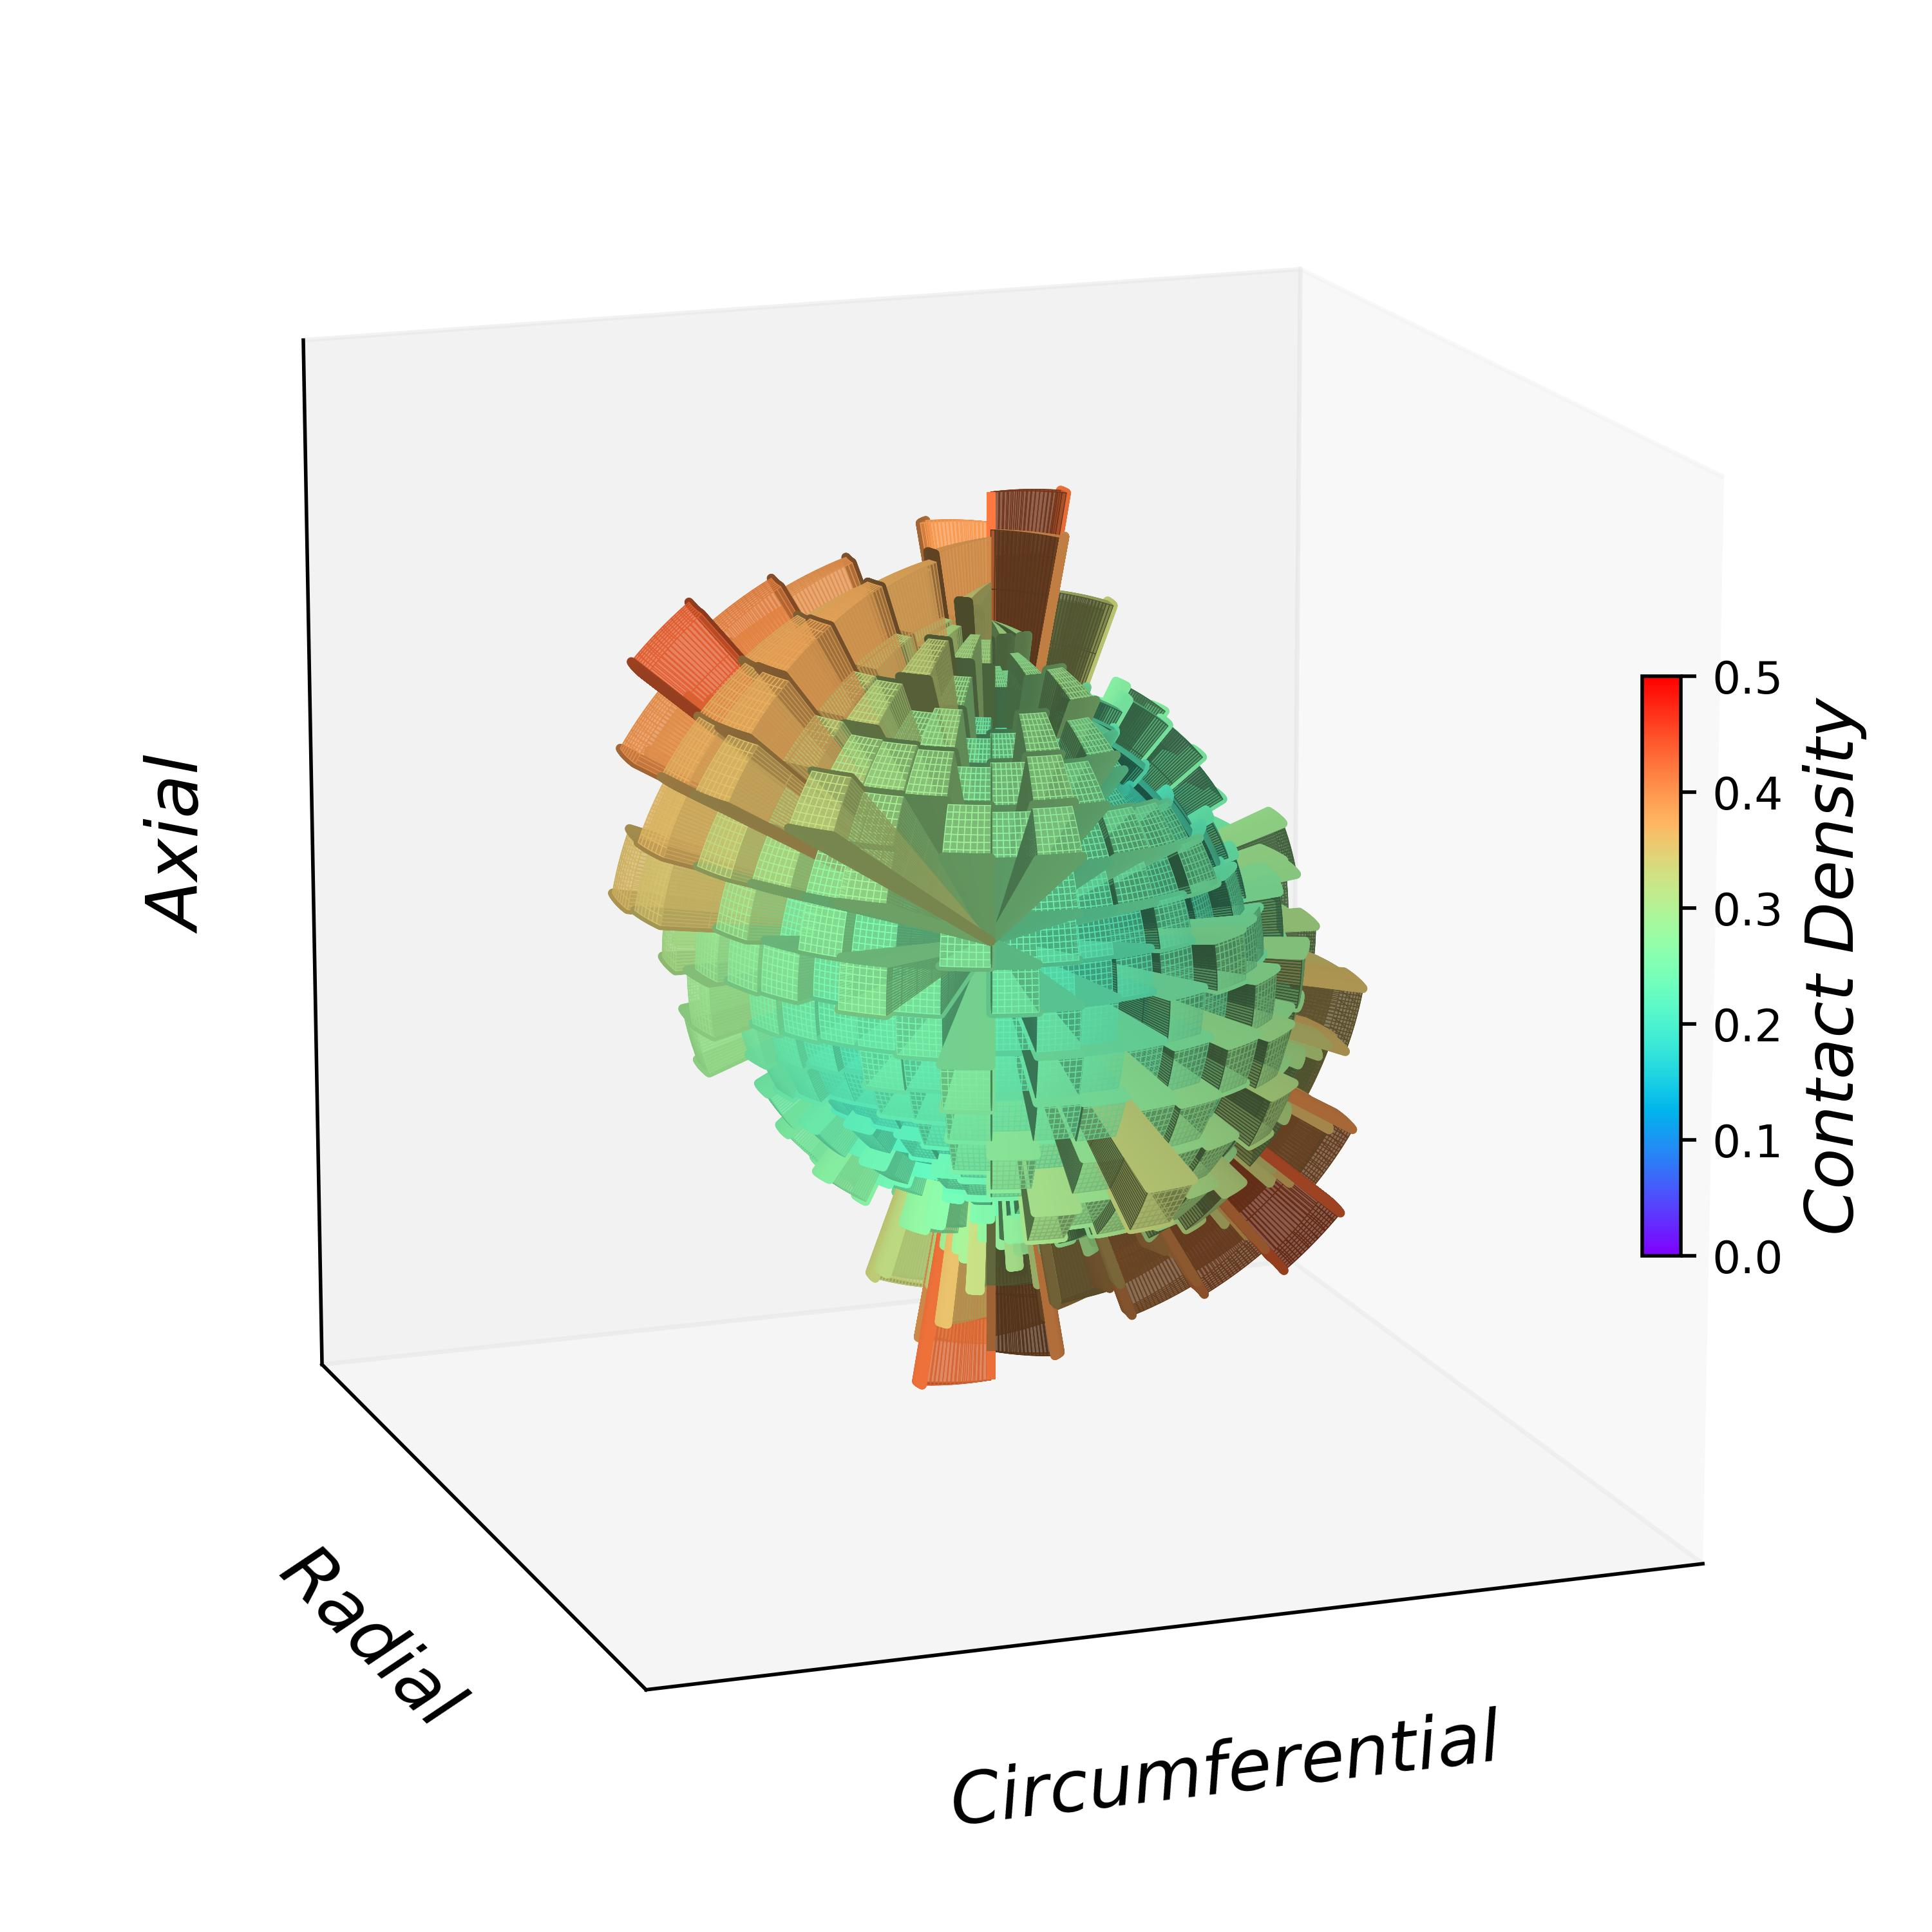
\includegraphics[width=\imgW]{contact_density_k0_20_t379.png}};
  \node[anchor=north west, inner sep=0] (b4) at ([xshift=\gap]b3.north east)
    {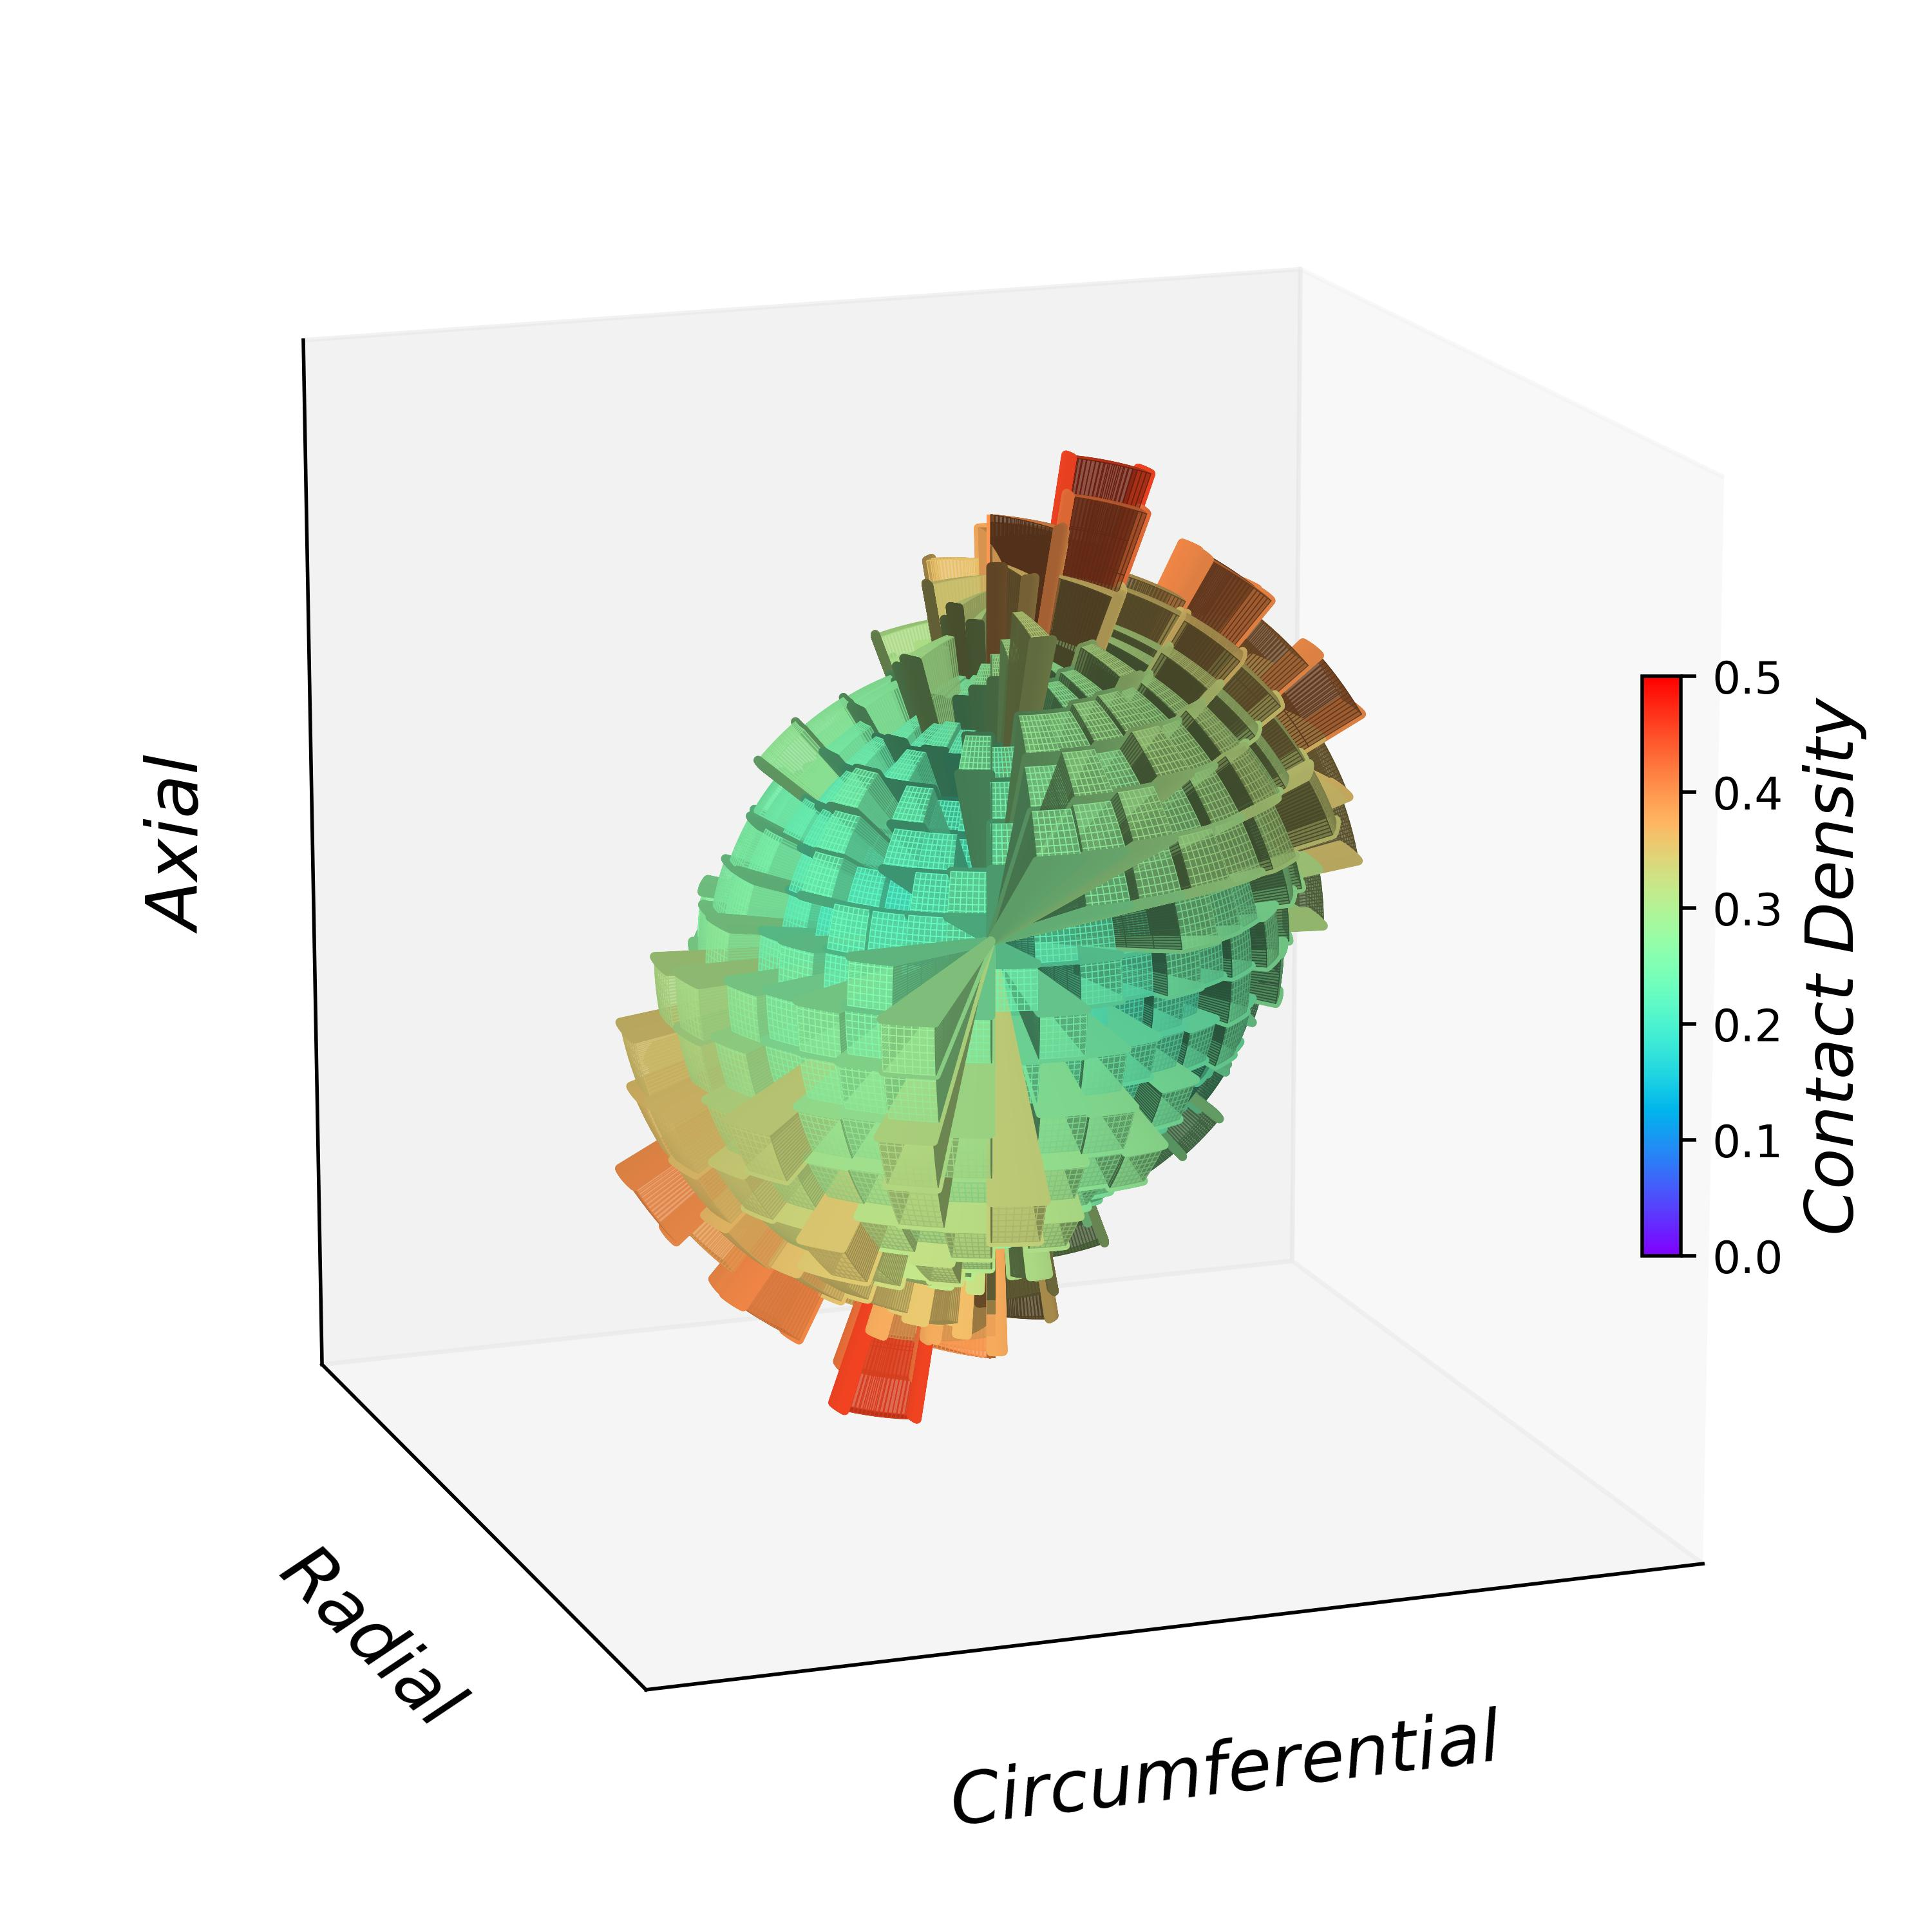
\includegraphics[width=\imgW]{contact_density_k0_20_t386.png}};

  % K0=2.0 label
  \path (b1.south) -- (b4.south) coordinate[midway] (row2mid);
  \node[font=\scriptsize, anchor=north] at ([yshift=-1pt]row2mid) {$\Kzero{} = 2.0$};

  % --- Rainbow colorbar (right, spanning both rows) ---
  \pgfpointdiff{\pgfpointanchor{b4}{south}}{\pgfpointanchor{a4}{north}}
  \pgfgetlastxy{\discard}{\cbarH}
  \node[anchor=north west, inner sep=0] (cbar) at ([xshift=4pt]a4.north east)
    {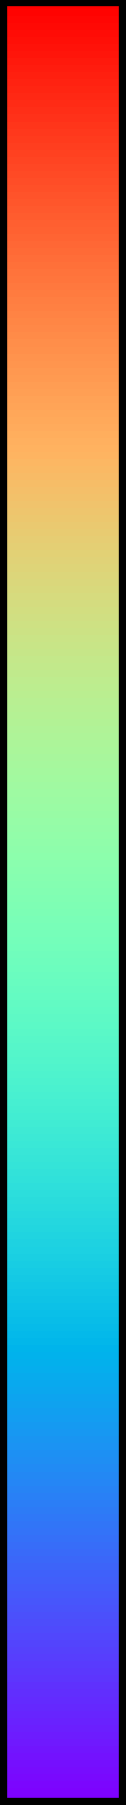
\includegraphics[height=\cbarH]{colorbar_rainbow.png}};
  \foreach \val/\frac in {0.5/0, 0.4/0.2, 0.3/0.4, 0.2/0.6, 0.1/0.8, 0/1.0} {
    \node[font=\footnotesize, anchor=west] at
      ([xshift=2pt, yshift={-\frac*\cbarH}]cbar.north east) {\val};
  }
  \node[font=\footnotesize, rotate=90, anchor=south] at
    ([xshift=32pt]cbar.east) {Contact density $\rho_c$};

  % --- DEBUG: uncomment grid to help position axis labels ---
  % \begin{scope}[
  %   x={(a1.south east)}, y={(a1.north west)}, shift={(a1.south west)},
  % ]
  %   \draw[help lines, step=0.1, gray!30] (0,0) grid (1,1);
  %   \foreach \x in {0.0, 0.1, ..., 1.0} {
  %     \node[font=\tiny, gray] at (\x, -0.02) {\x};
  %   }
  % \end{scope}
\end{tikzpicture}
\end{document}
